\chapter{Softwareimplementering}

\section{Version}
\begin{table}[h]
	\centering
	\begin{tabularx}{\textwidth - 2cm}{|l|l| l|X|}
	\hline
	Dato	& Version	& Initialer & Ændring	\\ \hline
	27. november & 1 & LS	& Første udkast af dokumentet \\ \hline
	\end{tabularx}
\end{table}


\section{PC blokken}
\subsection{Scenario (Kristian S.)}

\subsubsection{Scenario constructor}

Scenario klassen bruger STL(Standard Template Library) vector container format istedet for et array. Constructoren bruger STL's assign funktion til at oprette 20 aktion objekter med default værdier.

\subsubsection{getAction}

Metoden returner en reference til et aktion objekt i vectoren på baggrund af pladsen i den.

\subsubsection{sortActions}

sortActions bruger STL's sorterings funktionalitet til at sætte de aktions objekter i numerisk rækkefølge set i forhold til deres tids værdi. For at kunne sammenligne aktion objekter, har aktion klassen fået overloadet dens "<" operator. sortAction har ikke længere en returværdi, men muterer et scenarios vector af action objekter.

\begin{lstlisting}
void Scenario::sortActions()
{
		sort(scen_.begin(), scen_.end());
}
\end{lstlisting}

\subsubsection{clearActions}

clearActions bruger clear funktionen i STL for at slette alle actions objekter, hvor efter de bliver oprettet igen med default værdier.


\subsubsection{Ostream Operator}

Scenario klassens ostream operator er blevet overloadet til brug i UI klassen. "<<" operatoren udskriver nu alle aktion objekters værdier som: Tid, kommando og enhed.


\clearpage
\subsection{Action (Kristian S.)}

\subsubsection{Constructors}

Aktion klassen indeholder to constructors: En default constructor, der kaldes 20 gange når Scenario objektet først oprettes, og en explicit constructor til de prædefinere scenarier. 

\subsubsection{setUnit}

set-metode til at sætte aktionens enhedsværdi.

\subsubsection{setCommand}

Set-metode til aktionens kommandoværdi. Funktionen oversætter kommandoens talværdi til en char, der vil blive brugt i UART klassen.

\subsubsection{setTime}

Set-metode til aktionens tidsværdi.

\subsubsection{getUnit}

Get-metode til aktionens enhedsværdi.

\subsubsection{getCommand}

Get-metode til aktionens kommandoværdi.

\subsubsection{getTime}

Set-metode til aktionens tidsværdi

\subsubsection{ostream operator}

\texttt{Ostream} operatoren er overloadet og implementeret som en fri funktion, og kan derfor ikke tilgå de private members direkte.

\subsubsection{Less than operator}

Yderligere er der tilføjet en overload af operatoren \texttt{<}, så et Action objekt kan sammenlignes direkte på dens tids værdi.

\clearpage
\subsection{UI (Kasper)}

UI'en er en klasse der består af en række metode-kald. Hver af metoderne clearer skærmen for tidligere menu, og tegner den nye menu alt efter hvilken menu, der bliver kaldt. skærmen bliver clearet ved brug af kommando'en \texttt{system("cls")}. som forekommer i starten af alle metode-kaldene. En metode afsluttes ved at returnere en integere i alle tilfælde, men untagelse af funktionen \texttt{drawStopPromt} som returnerer en boolean.

\subsubsection{drawMainMenu}
drawMainMenu metoden udskriver en en liste over mulige menuer på skærmen hvorefter brugeren får mulighed for at indtaste, hvilken menu der ønskes. ved brug af \texttt{Cin} til at læse input fra brugeren, kan brugeren også indtaste forkerte inputs som f.eks. "AA3". Til at forhindre at forkerte inputs bliver indlæst, bliver der fortaget en validering af den indtastede int. Det tjekkes at inputtet er imellem 1 og 3, og alle andre inputs resultere i en fejlmeddelse på skærmen, og beder brugeren om at prøve igen.
\begin{lstlisting}
cin >> pick;
			if (pick >= 1 && pick <= 3) // tjekker at input vaerdien er indenfor gyldige graenser
				return pick;
			else
				cout << "ugyldig menu, pr\x9Bv igen: ";
\end{lstlisting}


Ved inputs som f.eks. "AA3", vil inputtet ikke kunne valideres ordenligt og resultere i en uendelig løkke af fejlmeddelser. Ved at flushe keyboardets buffer, sørges der for at uanset hvor lang en tekst brugeren indtaster, resultere det kun i en enkelt fejlmeddelse.
\begin{lstlisting}
cin.clear();
fflush(stdin);
\end{lstlisting}

\subsubsection{drawScenList}
Metoden \texttt{drawScenList} udskriver en liste med beskrivelsen af 3 forudindstillede scenarier. hvorefter brugeren kan vælge en af de forudindstillede scenarier. Validering af input og valg fungere på samme måde som \texttt{drawMainMenu} metoden.

\subsubsection{drawScenario}
Metoden \texttt{drawScenario} får en reference til et scenarie ind som parameter. Metoden bruger Scenariet ostream operater til at udskrive de 20 aktioner, der ligger i scenariet ud på skærmen.
\begin{lstlisting}
int drawScenario(Scenario & Scen) 
{	
	...
	cout << Scen;
\end{lstlisting}


Brugeren kan herefter vælge en af de 20 aktioner, ved at indtaste nummeret på aktionen. valg og validering af aktion fungerer på samme måde som \texttt{drawMainMenu}, dog er validering af input sat imellem 0 og 19, istedet for 1 og 3.
\begin{lstlisting}
if (pick >= 0 && pick <= 19)
\end{lstlisting}


\subsubsection{drawAskUnit}
metoden \texttt{drawAskUnit} udskriver en liste over Units der kan vælges til udførsel af en kommando. Brugeren kan vælge mellem 2 lamper, et TV og en radio. valg og validering af input fungere på samme måde som \texttt{drawMainMenu}, dog er validering af input sat imellem 1 og 2, som er de 2 lamper. TV og Radio kan ikke vælges, da de ikke implementeres i systemet.

\subsubsection{drawAskCommand}
metoden \texttt{drawAskUnit} udskriver en liste over kommandoer der kan udføres af den givne Unit. brugeren kan vælge mellem at tænde, slukke og dimme. Valg fungere som i \texttt{drawMainMenu} metoden. Validering af input tjekker her for om det er enten tænd, sluk eller dim der er valgt. Ved tænd og sluk returnere koderne for det valgte, men hvis det valgte er dim, får brugeren mulighed for at vælge styrken af dimming. Styrken af dimming valideres og returneres. Hvis brugeren indtaster en værdi uden for det gyldige område, bliver metoden kørt fra begyndelsen, hvor tænd, sluk eller dimming skal vælges igen.



\subsubsection{drawAskTime}
metoden AskTime fungere ved at brugeren bliver bedt om at indtaste hvilket time-tal på dagen den ønskede kommando skal udføres på. Herefter bliver brugeren bedt om at indtaste det ønskede minut-tal på den valgte time. Tiden valideres, og hvis både time-tal og minut-tal er indenfor de gyldige grænser returneres tiden siden midnat i minutter. $timer*60+minutter$ 
Hvis enten time-tal eller minut-tal er udenfor de gyldige grænser, får brugeren besked om at den indtastede tid er ugyldig og keyboard-bufferen tømmes. Når en en knap trykkes ved fortsættes programmet, og metoden bliver startet forfra. Til at vente på en knap trykkes er brugt \texttt{\_getch()} som kan bruges til at hente hvilken knap på keyboardet er trykket. I dette tilfælde er funktion brugt til at tjekke om en knap bliver trykket på, og ikke for at gemme inputtet af hvad der er trykket på.
\begin{lstlisting}
if (hour >= 0 && hour <= 23 && min >= 0 && min <= 59)
				return (hour * 60 + min); // returnere tiden siden kl 00
			else
				cout << "ugyldig tid, pr\x9Bv igen";
			
			cin.clear();
			fflush(stdin); //clear og flusher alt gemt i keyboard bufferen
			_getch(); //venter paa hvilket somhelst tryk paa keyboard
\end{lstlisting}


\subsubsection{drawStopPromt}
drawStopPromt metoden udskriver på skærmen en besked om brugeren er sikker på at afviklingen af scenarie skal afsluttes. Ved at trykke på knappen "Y/y" på keyboardet, bekræftes det at det skal afsluttes og der returnes \texttt{true}, en hver anden knap resultere i, at der returneres \texttt{false}
\begin{lstlisting}
get = _getch();
if (get == 89 || get == 121) // ascii vaerdi for y og Y
			return true;
		else
			return false;
\end{lstlisting}

\clearpage
\subsection{PC UART (Kasper)}

PC'ens UART har til formål at oversætte de data, der er i \textit{Scenario}-objektet, og transmittere dem over på transmitteren. Dette gøres ved brug af et open-source bibliotek kaldet RS232\cite{lib:UART}, der følger den protokol det ønskes at transmittere data med.

For at sende data ud til Transmitteren, skal der oprettes en forbindelse gennem en USB port. her bruges \texttt{UART\_connect} til formålet.

Systemet kræver også at kunne få status på kodelåsen, hvilket metoden \texttt{getLockStatus} står for. Kravet for at bruge \texttt{getLockstatus} er, at \texttt{UART\_connect} har været kørt, for at finde en gyldig port at sende og modtage på.

Når data skal transmitteres bruges \texttt{sendScen}, der tager en reference til et scenarie som parameter, og får oversat dataene i scenariet til at følge UART protokollen, hvorefter den sender dem over til transmitteren.


\subsubsection{UART\_connect}
Metoden \texttt{UART\_connect} bruges til at finde en gyldig COM-port på computeren. Metoden kører igennem alle COM-porte på PCen ved at bruge RS232-bibliotekets funktion \texttt{RS232\_openComport}, til at tjekke om der sidder et RS232 stik i den givne COM-port. Så længe den testede COM-port ikke har et RS232 stik i, tæller metoden Cport\_nr en op, og derved tester den næste COM-port, indtil en gyldig COM-port er fundet.

\begin{lstlisting}
while (RS232_OpenComport(cport_nr, bdrate, mode))
		{

			printf("ugyldig Com-port\n");
			cport_nr++;
		}
\end{lstlisting}

\subsubsection{getLockStatus}
Metoden \texttt{getLockStatus} finder ud af kodelåsens status ved at sende et \texttt{L} ud på COM-porten. Dette sker ved at bruge RS232-bibliotekets funktion \texttt{RS232\_cputs()}. Parametrene for funktionen er COM-port nummeret \texttt{cport\_nr} og den mængde af data i form af chars, der skal sendes.\\
Da det kræver COM-port nummeret, er det derfor også nødvendigt, at metoden \texttt{UART\_connect} har været kørt, før det er muligt at bruge \texttt{getLockStatus}.

\begin{lstlisting}
RS232_cputs(cport_nr, "L");
\end{lstlisting} 

Når beskeden om at tjekke status er blevet sendt til transmitteren, begynder metoden at læse på porten og venter på et svar tilbage fra transmitteren. Svaret vil indeholde et \texttt{L} eller et \texttt{U}, afhængig af om kodelåsen er hhv. låst eller oplåst. Til aflæsning på COM-porten bruges RS232-bibliotekets funktion \texttt{RS232\_PollComport()}.
Hvis det aflæste er et \texttt{L} returneres \texttt{true}, for at kodelåsen er låst. Hvis et \texttt{U} aflæses returneres \texttt{false}, hvilket betyder kodelåsen er låst op.

\subsubsection{sendScen}
metoden Send Scen har til opgave at oversætte data fra scenariet til chars som følger UART protokolen.
til at starte med kører metoden koden nedenfor:
\begin{lstlisting}
RS232_cputs(cport_nr, "N");
\end{lstlisting} 
\texttt{N}'et betyder at transmitteren skal være klar på at der nu kommer et ny datastrøm fra PCen. 
Metoden henter herefter den første aktion, så \texttt{get} funktioner kan bruges til at hente data ud af aktionen.
Kommandoen bliver sat direkte ind, da \texttt{get} funktionen for den returnerer en char, derfor sker ingenting med den. 
Tiden skal regnes om, så transmitteren ved hvor længe der skal gå, før den skal udføre en kommando. Dette sker i koden set nedenfor:
\begin{lstlisting}
				//udregner tiden til den gaeldne commando skal ekseveres
				int timeTillExecution;
				if (action.getTime() >= Ctime())
				{
					timeTillExecution = action.getTime() - Ctime();
				}
				else
				{ 
					timeTillExecution = 1440 - (Ctime()-action.getTime()); 
				}
				//tager sig af at omregne tiden fra int til char og dele tiden op i 2 chars, da den kan ske at fylde mere end 8 bit
				int timeL1 = timeTillExecution % 16; 
				int timeL2 = int((floor(timeTillExecution / 16) % 16)
				int timeH = int((floor(timeTillExecution / 256)));

				TimeLow1 = ((char)timeL1 +48);
				TimeLow2 = ((char)timeL2+48)
				TimeHigh = ((char)timeH)+48);
\end{lstlisting} 
Integeren \texttt{timeTillexecution} bliver udregnet ud fra en af 2 udregning. Den valgte udregning afhænger af om tidspunktet allerede har passeret systems klokkeslet. Hvis dette er tilfældet køres udregningen i linje 9. Denne udregning tager hensyn til hvor mange minutter der er tilbage på dagen og kører derfor på det angivne klokkeslet næste dag. udregningen i linje 5 sker hvis klokkeslettet endnu ikke har passeret tiden, hvor kommandoen skal udføres. Den udregner hvor mange minutter der er fra det gældende klokkeslet og frem til kommandoen skal udføres.
\texttt{Ctime()} funktionen som fremgår flere steder er en hjælpefunktionen som returnerer en integer med klokkeslettet på PCen.
Når \texttt{timeTillExecution} er udregnet, skal den omsættes til Chars. Da den maksimale værdi der vil fremkomme er 1440(antallet af minutter på et døgn), skal der bruges 2 chars til at gemme dataene i.
\begin{lstlisting} 
				int timeL1 = timeTillExecution % 16; 
				int timeL2 = int((floor(timeTillExecution / 16) % 16)
				int timeH = int((floor(timeTillExecution / 256)));
\end{lstlisting} 
\texttt{timeL1} er hvor de 4 første bit gemmes, derfor tages modulus til 16 for at finde resten, og altså den værdi der skal gemmens i \texttt{timeL1}.
\texttt{TimeL2} er hvor de midterste bit gemmes, derfor nedrundes der,og denne omskrives til en int. Derefter tages modulus til 16.
\texttt{timeH} er hvor de 4 største bit gemmes. For at finde værdien der skal gemmes heri, divideres \texttt{timeTillExecution} med 256, og rundes ned, for præcision. Da nedrundingen sker som en double omskrives det til en int, efter nedrundingen.

\texttt{timeL1}, \texttt{timeL2} og \texttt{timeH} har efter udregningen en makimalstørrelse på 16, og kan derfor laves om til en char, med ASCII kode mellem 48 og 64
\begin{lstlisting} 
				TimeLow1 = ((char)timeL1 +48);
				TimeLow2 = ((char)timeL2+48)
				TimeHigh = ((char)timeH)+48);
\end{lstlisting} 

Unit oversættes ved brug af en switch set i koden nedenfor:
\begin{lstlisting} 
switch (action.getUnit()) // tager sig af at oversaette unit til at foelge UART protocollen
			{
			case 1:
				unit = 'A';
				break;
			case 2:
				unit = 'C';
				break;
			case 3:
				unit = 'P';
				break;
			case 4:
				unit = 'N';
				break;
			default: 
				unit = '0';
				break;

			}
\end{lstlisting} 
Switchen tager uniten ind fra aktionen, og alt efter værdien sættes unit til den char der passer en den gældende unit.

UARTen sender nu dataene fra aktionen ud på COM-porten ved brug af funktionen \texttt{RS232\_cput}

\begin{lstlisting}
char data[6] = { unit, command, TimeHigh, TimeLow2, TimeLow1 }; // data der skal sendes over
			strcpy(str[c], data);
			RS232_cputs(cport_nr, str[c]);
\end{lstlisting}

når dataene er sendt på på porten, venter UARTen 100milisekunder, hvorefter den begynder forfra med aktion nr.2. Dette sker til alle 20 aktioner er overført til transmitteren, hvorefter metoden afslutter.


\subsubsection{stopAll}
metoden \texttt{stopAll} er til at slukke alle enheder på system. Dette gør metoden ved at bruge funktionen \texttt{RS232\_cput} til at sende et \texttt{S} til transmitteren. Transmitteren ved ifølge protokolen at et \texttt{S} betyder den skal slukke alt.
\begin{lstlisting}
RS232_cputs(cport_nr, "S");
\end{lstlisting}
\subsection{PC Main (Henrik)}
PC'ens main har til formål at stykke alle PC'ens klasser sammen, og styrer alt fra input til output. Den er kodet således at UC1, UC2 og UC3 er opfyldt. Basalt set er dette en main fil som bruger alle funktioner fra PC'ens klasser: Action, PC UART, Scenario og UI.\\
Ud over dette er det under denne fil at koden til de predefinerede scenarier ligger.\\
\clearpage

%Skrevet af David
\section{Generelt om Microcontrollers (David)}
I vores projekt har vi valgt at bruge Atmels ATMega32 microcontroller, fordi vi har kendskab til netop denne via MSYS kurset på første semester, den blev også brugt til vores bil på selv samme semester.

\subsection{C++}
I vores projekt har vi valgt at programmere i C++ frem for C. På microcontrolleren får vi den store fordel at vi kan opbygge alt i klasser frem for frie funktioner.

Dette er valgt for gør det nemmere for os som udviklere at kode hver klasse, og kun have den logik, som skal bruges i denne. Dette gør det nemmere at teste koden, samt at dele softwareopgaverne ud blandt flere personer, fordi at så længe klassen overholder vores designdokument, er det nemt at sætte det hele sammen til sidst, hvor alt kode er skrevet.

Dette giver os den store fordel at vi kan gøre brug af de såkaldte ''The Three Pillars of Object-Oriented Programming'' (indkapsling, arv og polimorfi), hvor det giver mening.

Vi gør dog kun rigtig brug af Encapsulation da vi ikke har vurderet at, der var nogen steder det ville give mening at anvende Inheritance og Polymorphism. 
Encapsulation giver rigtig meget mening for os, da information hiding hjælper med at beskytte vigtigt private data, som eksisterer eksempelvis i vores boundry klasser til X.10 kommunikation. 
I praksis betyder det at kun klassens egen metoder må ændre dets private data. Dette er rigtig smart fordi at man så er helt sikker på at der ikke bliver unødigt eller fejlagtigt ændret i en variable som potentielt kan ødelække klassens funktionalitet.

\subsection{C++ Compiler på Microcontrollerne}\label{sec:micro}
Da vi skulle undersøge hvordan man kunne anvende C++ på vores microcontroller, så vi først på Atmels hjemmeside\cite{lib:atmel} for at finde ud af om der er nogle ting der skal gøres specielt opmærksomt på. Vi startede med at skrive vores kode inline, da der har været god erfaring i gruppen med at gøre det i Visual Studio 2013, dog viste dette sig at give massive problemer når der blev kodet inline i Atmel Studio 6.2. Problemerne var bl.a. at indlæse variabler, som blev erklæret i toppen af dokumentet, men længere nede i metoderne. Derfor blev det vedtaget, at der skulle bruges den klassiske struktur med adskilte header og .cpp filer.

\subsection{C++ og Interrupts}
Der var ingen i gruppen, der havde kendskab til hvordan interrups på microcontrollerne i C++ fungerede, derfor blev der hentet inspiration fra et open source projekt\cite{lib:waterproofman}. Det viste sig at fungere ganske godt og uden de store problemer og gruppen var på kort tid i stand til at opstille en test med interrupts i C++.

\subsection{C++ på AVR Object Kommunikation}
Normalt kan objekter oprettes i en seperat cpp fil, hvorefter man kan anvende dot-operatoren til at tilgå et objekts metoder og variable. Dette fungerede ikke i Atmel Studio 6.2, da compileren ikke kunne finde de givne objekter, derfor var man nød til at lade de objekter der skulle interagere med hinanden via en fri funktion, der returnerede en pointer til det givne objekt.

\clearpage

%Skrevet af Kristian T, undtagen time klassen, som er skrevet af Kristian S.

\section{Transmitter Blokken}

\subsection{Action Klassen (Kristian T.)}

Selve \texttt{Action}-klassen består af en række get'er metoder og én set motode, som validerer data og genererer \texttt{houseCode} ud fra \texttt{unitCode} parametren. Der er ikke foretaget nogle videre interessante algoritmer eller yderligere hjælpefunktioner udover dem, der forefindes i kapitlet Software Design.

\subsection{Codelock Klassen (Kristian T.)}

Implementeringen af denne klasse er blot én metode \texttt{locked()}, som returnerer true, hvis kodelåsen er låst (benet er højt).

\begin{lstlisting}
bool Codelock::unlocked(){
	//TRUE if unlocked, FALSE is locked. 
	//Signal is LOW when code is correct, HIGH when not correct.
	return !(PINA & 0b0000001);
}
\end{lstlisting}

\subsection{Time Klassen (Kristian S.)}

Time klassens roller er at give TransmitterCtrl klassen en opdateret værdi i minutter hver 5 sekund. Dette tager højde for flere events, som vil kører på samme tid og giver Tx10 klassen mulighed for at sende hele aktionen før næste aktion påbegyndes. Klassen er blevet implementeret med en compare interrupt på Timer1, hvor der sker et overflow hvert sekund, som inkrementer en \texttt{seconds} variabel. Når denne \texttt{seconds} er modulo 0 med 5, sendes \texttt{minutes} til ctrl klassen, ellers hvis \texttt{second} overstiger 59 bliver den sat til 0 og \texttt{minutes} tillægges 1. 

\begin{lstlisting}
ISR(TIMER1_OVF_vect){
	
	//increments the time by 1 sec
	myTime.seconds++;
	
	//every 60 seconds updates Minutes value.
	if(myTime.seconds > 58){
	    myTime.seconds = 0;
		myTime.minutes++;
	}
		
	//every 5 seconds updates transmitters next action time.
	if(myTime.seconds % 5 == 0){
		myTime.myTransPtr->checkTime( myTime.minutes );
	}
}
\end{lstlisting}

\subsection{Transmitter Klassen (Kristian T.)}

\subsubsection{Constructor}
Til implementering af Transmitter klassen er der lavet en constructor, som initierer de to variabler \texttt{charCounter} og \texttt{scenCounter}. Udover dette opretter den et array på 20 pladser, som den fylder med tomme \texttt{Action} objekter.

\subsubsection{scenData(char input)}
Denne metode er implementeret, så den tjekker hvor mange dele af en \texttt{Action}, der er gemt og når et helt \texttt{Action} objekt er overført, gemmes dette i objekt nummer \texttt{scenCounter}, som holder styr på hvor mange \texttt{Action} objekter der er overført. Når data gemmes oversættes den samtidigt til de kodemønstre, som X10 protokollen bruger.

\subsubsection{checkTime(unsigned int theTime)}
Denne metode er implementeres således at den kaldes sig selv rekursivt for at tjekke om der er flere aktioner oprettet på samme tidspunkt. Hvis dette er tilfældet fortsætter den med rekursive kald, indtil der ikke er flere aktioner til tidspunktet eller at alle aktioner i hele scenariet er blevet udført (i det tilfælde, hvor alle aktioner i et scenarie ligger samtidigt).

\begin{lstlisting}
void Transmitter::checkTime(unsigned int theTime){
	if (myScenario[nextAction].getTime() == theTime){ //Check to see if the time has past the next action to be sent
		if (firstLoop){					//Check if this is the first recursive call
			breakAt = nextAction;		//Set the breaking point for recursive calls
			firstLoop = false;
		}
		else{
			if (breakAt == nextAction){	//Check if the breaking point has been reached
				firstLoop = true;
				return;					//Break out of the recursive calls, if all the actions in the Scenario have been sent simultaniously
			}
		}
		myTx10Ptr->sendAction(myScenario[nextAction]);
		nextAction++;
		if (nextAction == 20){ //If the last action has been sent, queue the first action
			nextAction = 0;
		}
		checkTime(theTime);		//Recursive call, to check if several actions are on the same time.
	}
	else
	firstLoop = true;
}
\end{lstlisting}

\subsection{Tx10 Klassen (Kristian T.)}

Klassen fungerer ved at der hele tiden kommer interrupts fra \texttt{zeroCrossDetected} signalet, 100 interrupts i sekundet. Datamedlemmet \texttt{bool start} bestemmer om \texttt{Tx10} klassen, skal sende noget ud på nettet eller ej.

\subsubsection{Constructor}
Constructoren sørger for at initialisere samtlige variabler til værdier, som giver mening. Den initialiserer Timer0, Timer2 og INT0 samt PORTC til debugging med LED-lysene, som sidder på STK500.

Timer0 bruges til at danne et 120 kHz clocksignal, til at beregne de initierede værdier er følgende udregninger lavet. Dette er når $f_{osc} = 3.6864 \text{MHz}$, $N = 1$ og $OCR0 = 14$. 

\begin{displaymath}
f = \frac{f_{osc}}{2 N (1 + OCR0)} = 122.88 \text{kHz}
\end{displaymath}

\subsubsection{unsigned char Translate(unsigned char bitCode)}

Hjælpemetode, som oversætter 4-bit tal til en char indeholdende 8 nulgennemgange. Denne er implementeret med \texttt{if}-sætninger, som tjekker på de enkelte bits i \texttt{bitCode}.

\begin{lstlisting}
unsigned char Tx10::translate( unsigned char bitCode ){
	unsigned char temp = 0;
	if (bitCode & 0b00001000){
		temp |= 0b10000000;
	}
	else{
		temp |= 0b01000000;
	}
	if (bitCode & 0b00000100){
		temp |= 0b00100000;
	}
	else{
		temp |= 0b00010000;
	}
	if (bitCode & 0b00000010){
		temp |= 0b00001000;
	}
	else{
		temp |= 0b00000100;
	}
	if (bitCode & 0b00000001){
		temp |= 0b00000010;
	}
	else{
		temp |= 0b00000001;
	}
	return temp;
}
\end{lstlisting}

\subsubsection{sendAction(Action \&)}
Metoden starter med at gemme \texttt{Housecode}, \texttt{Unitcode} og \texttt{Command} fra aktionen i \texttt{Tx10} klassens egne variabler ved hjælp af \texttt{Translate()} og sætter \texttt{start} til \texttt{TRUE}.

\subsubsection{sendCrossing(unsigned char send)}

Hjælpemetode, som åbner op for 120 kHz firkantsignal, hvis send er forskellige fra 0.

Metoden er testet til at give outputtet i Figur \ref{fig:sendCrossingtest} på STK500 når den kaldes med en char forskellige fra 0. 

\begin{figure}[h]
\centering
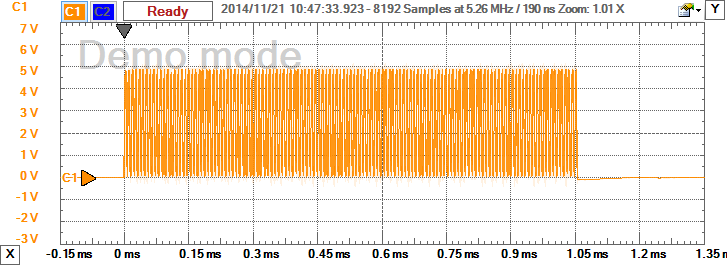
\includegraphics[width=\textwidth]{../Implementering/SW_implementering/Transmitter/sendCrossing_test}
\caption{Output på X.10Data når en der skal sendes 1 i en nulgennemgang.}
\label{fig:sendCrossingtest}
\end{figure}

Frekvensen på firkantsignalet er med Analog Discovery målt til 122 kHz.

\subsubsection{waitMs()}

Hjælpemetode, som starter timer2 på 1 ms og venter til denne er færdig inden metoden forlades. 

Tiden er regnet ud ud fra følgende formel:

\begin{displaymath}
t = \frac{1}{f_{osc}} N (C - 1) = 1.00 ms
\end{displaymath}

Hvor $N$ er sat til 64 og $C$ er sat til 59. $N$ er prescaleren på clockfrekvensen for ATMega32 og $C$ er antallet af tællinger der skal til. Dvs at der skal skrives $255 - C$ til OCR2 registreret.

\subsubsection{intHandler()}

Hjælpemetode, som håndterer interrupts fra \texttt{zeroCrossDetected} benet. 

Starter med at tjekke om \texttt{start} er \texttt{TRUE}, hvis den er det fyldes \texttt{buffer} variablen med de næste nulgennemgange, som skal sendes. 

Starter med at sende MSB fra bufferen og skifte bufferen til venstre, indtil at bufferen er tom (\texttt{buffCount == 0}). Afhængigt af hvor mange mønstre (\texttt{pattCount}), som er sendt fylder den det næste mønster i bufferen. Når alle mønstre er sendt sætter den \texttt{start} til \texttt{false}.

\begin{lstlisting}
void Tx10::intHandler(){
	if (start){ //check if the Tx is supposed to transmit
		if (buffCount == 0){
			if (pattCount == 0){
				buffer = 0b11101111;
				buffCount = 4;
			}
			else if (pattCount == 1){
				buffer = house;
				buffCount = 8;
			}
			else if (pattCount == 2){
				buffer = unit;
				buffCount = 8;
			}
			else if (pattCount == 3){
				buffer = command;
				buffCount = 8;
			}
			else if (pattCount == 4){
				buffer = 0b00000011;
				buffCount = 6;
			}
			else if (pattCount == 5){
				buffer = house;
				buffCount = 8;
			}
			else if (pattCount == 6){
				buffer = unit;
				buffCount = 8;
			}
			else if (pattCount == 7){
				buffer = command;
				buffCount = 8;
			}
			else if (pattCount == 8){
				buffer = 0b11110000;
				buffCount = 4;
			}
			else if (pattCount == 9){
				start = false;
				pattCount = 0;
			}
			pattCount++;
		}
		
		if (buffCount > 0){
			sendCrossing((buffer & 0b10000000)); //Send out the MSB
			buffCount--;
			buffer = (buffer << 1); //shifts the buffer one time to the left
		}
	}
	PORTC = ~getMyTx10()->buffer; //For debugging
}
\end{lstlisting}

\subsubsection{turnAllOff()}
Metode der fylder \texttt{house} variablen med 0 (koden for at slukke alt) og sætter \texttt{start} til \texttt{TRUE}. Dette medfører at ved de eftefølgende nulgennemgange sender mønstret for at slukke alt på nettet.

\subsection{TxUART Klassen (Kristian T.)} \label{TxUART}

Denne klasse er overordnet implementeret til brug i projektet ved overførsel af scenarier, men bruges også til dels til debugging af de øvrige klasser.

\subsubsection{Constructor}

Constructoren sørger for at initiere \texttt{mode} til \texttt{'i'} (idle) og initierer ellers UART på almindelig vis i henhold til protokollen.

\subsubsection{rxInt()}

Hjælpemetode, som håndterer interrupts når der modtages en \texttt{char} på UARTen. Metoden er implementeret ved at den kontrollerer hvilken tilstand, klassen er i. Hvis den er i idle udføres den kommando, som er sendt via UART. Hvis den er i receiving mode og der ikke er send 80 chars endnu, sendes der data til \texttt{Transmitter} klassen.

\begin{lstlisting}
void TxUART::rxInt(){
	char input = UDR;
	if (mode == 'i'){
		if (input == 'L'){
			bool temp = myTrans->getLockStatus();
			if (temp)
				sendChar('U');
			else
    			sendChar('L');
		}
		else if (input == 'N'){
			mode = 'r'; //put in receiving mode
			myTrans->newScen();
		}
		else if (input == 'S'){
			myTrans->stopAll();
		}
	}
	else if (mode == 'r'){
		if (charNo <= 80){
			myTrans->scenData(input);
			charNo++;
		}
		if (charNo == 80){ //end of data
			charNo = 0; //reset counter
			mode = 'i'; //put in idle mode
		}
	}
}
\end{lstlisting}

\subsubsection{sendChar(char)}

Hjælpemetode, sender en char via UART.

\subsubsection{sendString(const char * sendMe)}
Hjælpemetode til debugging, sender en række chars via UART, modtager "string literal", som de forekommer i C++. Dvs man fx kan skrive \texttt{sendString("Hello world.")}.

\subsubsection{sendNumber(int sendMe)}
Sender en integer via UART, som oversættes til ASCII-værdier først. Bruges primært til debugging af systemet.
\begin{lstlisting}
void TxUART::sendNumber(int sendMe){
	sendChar(((sendMe / 1000)%10)+48);
	sendChar(((sendMe / 100)%10)+48);
	sendChar(((sendMe / 10)%10)+48);
	sendChar(((sendMe)%10)+48);
}
\end{lstlisting}
\clearpage

\section{Receiver blokken}

\subsection{Lampe (David)}

\begin{figure}[h]
\centering
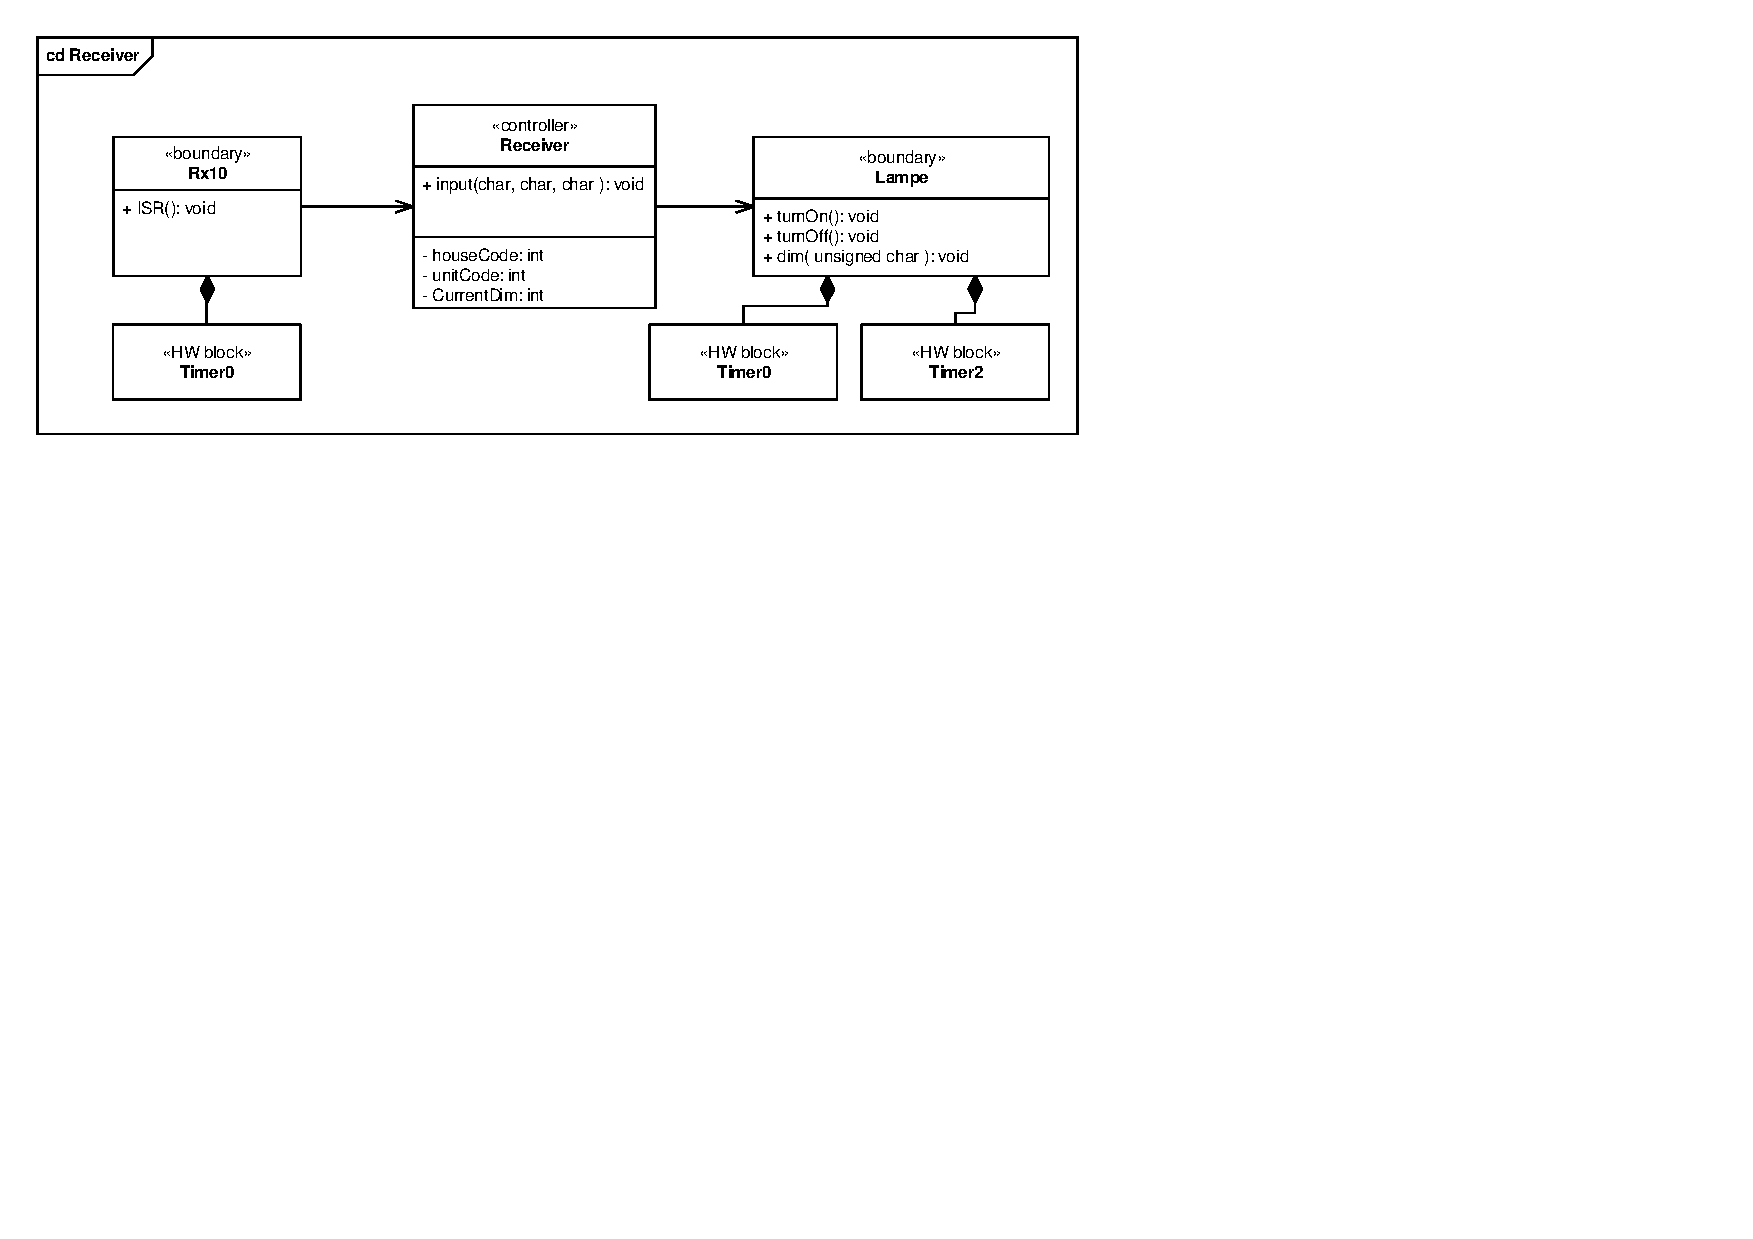
\includegraphics[scale=1,clip=true, trim=361.8 462 335 50]{Systemarkitektur/diagrammer/Receiver_KlasseDiagram} %L B R T - HUSKE DET
\end{figure}

\begin{table}[h]
\begin{tabularx}{\textwidth}{p{0.6 cm} l X} %\hline

%turnOn
\multicolumn{3}{l}{\textbf{turnOn}}\\
& Operation: & %Skriv tekst herunder
\texttt{void turnOn( void )}
\\ & Parametre: & %Skriv tekst herunder
Ingen.
\\ & Returværdi: & %Skriv tekst herunder
Ingen.
\\ & Beskrivelse: & %Skriv tekst herunder
Sætter PWM for lampen til 100\%.

\\ \end{tabularx}
\end{table}

%turnOff
\begin{table}[h]
\begin{tabularx}{\textwidth}{p{0.6 cm} l X} %\hline

\multicolumn{3}{l}{\textbf{turnOff}}\\
& Operation: & %Skriv tekst herunder
\texttt{void turnOff( void )}
\\ & Parametre: & %Skriv tekst herunder
Ingen
\\ & Returværdi: & %Skriv tekst herunder
Ingen
\\ & Beskrivelse: & %Skriv tekst herunder
Sætter PWM for lampen til 0\%.

\\ \end{tabularx}
\end{table}

\clearpage

%dim
\begin{table}[h]
\begin{tabularx}{\textwidth}{p{0.6 cm} l X} %\hline

\multicolumn{3}{l}{\textbf{dim}}\\
& Operation: & %Skriv tekst herunder
\texttt{void dim ( char )}
\\ & Parametre: & %Skriv tekst herunder
Modtager en char med en char med den ønskede dimnings værdi.
\\ & Returværdi: & %Skriv tekst herunder
Ingen
\\ & Beskrivelse: & %Skriv tekst herunder
Modtager en char som har en værdi mellem 0 og til og med 9, hvor 0 = 5\%, 1 = 15\% osv. Skal herefter ændre pulsbredden på det ben der er forbundet til lampen i forhold til den ovenfor angivne procent.
\\ \end{tabularx}
\end{table}

\subsection{Receiver (David)}

\begin{figure}[h]
\centering
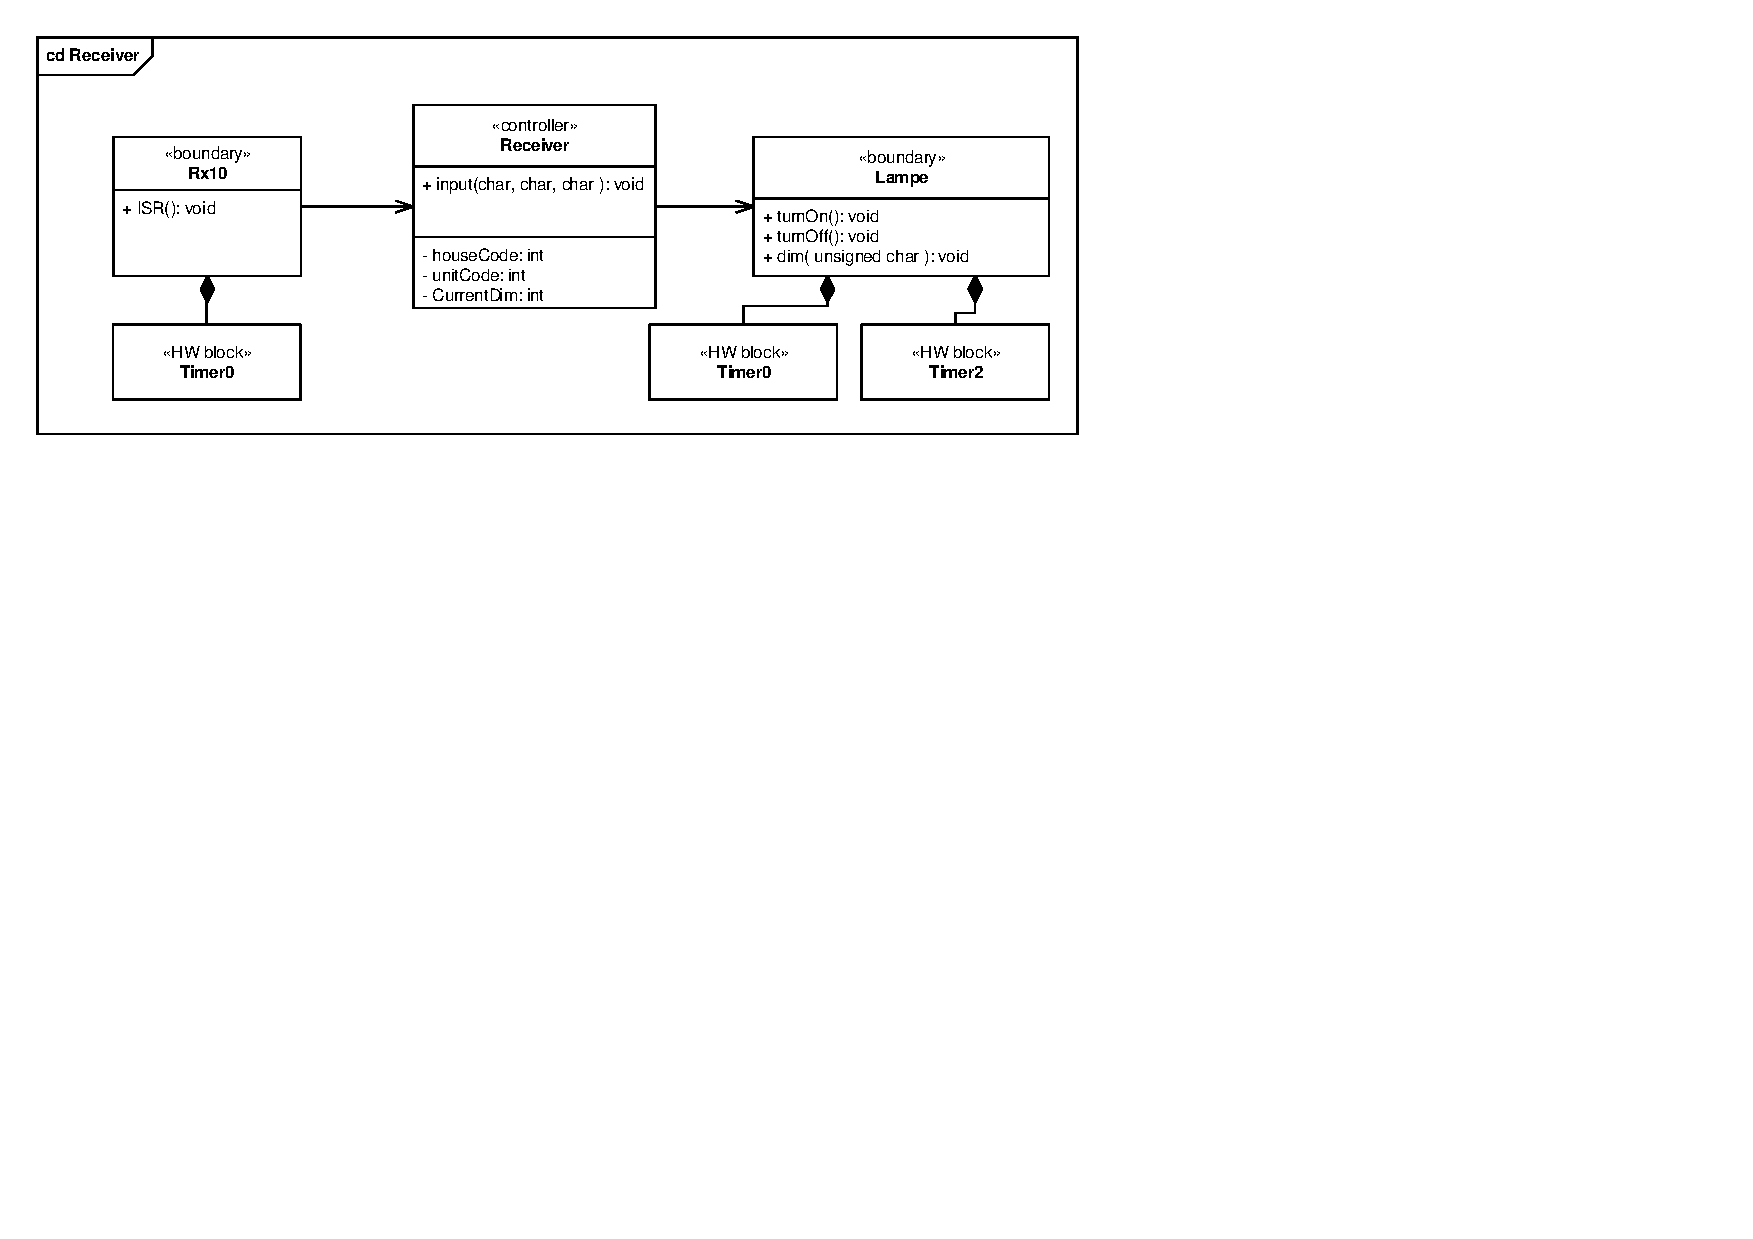
\includegraphics[scale=1,clip=true, trim=198 440 527 50]{Systemarkitektur/diagrammer/Receiver_KlasseDiagram} %L B R T - HUSKE DET
\end{figure}

\begin{table}[h]
\begin{tabularx}{\textwidth}{p{0.6 cm} l X} %\hline
\multicolumn{3}{l}{\textbf{Receiver}}\\
& Operation: & %Skriv tekst herunder
void input( char ) 
\\ & Parametre: & %Skriv tekst herunder
Modtager en char fra X.10 som bruges til at finde om lampen skal. Tænde, slukke, dime op, eller dime ned.
\\ & Returværdi: & %Skriv tekst herunder
ingen retur værdi. 
\\ & Beskrivelse: & %Skriv tekst herunder
Controller for receiveren. Holder styr på lampen nuværerne dimning samt dens houseCode og unitCode.
\\ \end{tabularx}
\end{table}

\begin{table}[h]
\centering
\begin{tabularx}{13 cm}{|l |X|} \hline
Attribut & Beskrivelse \\ \hline

houseCode & Indeholder hus koden for denne Receiver \\ \hline
unitCode  & Indeholder unit koden for denne Receiver \\ \hline
CurrentDim & Den nuværerne dim værdi. \\ \hline

\end{tabularx}
\end{table}

\clearpage

\subsection{Rx10 (Kristian T.)}

\begin{figure}[h]
\centering
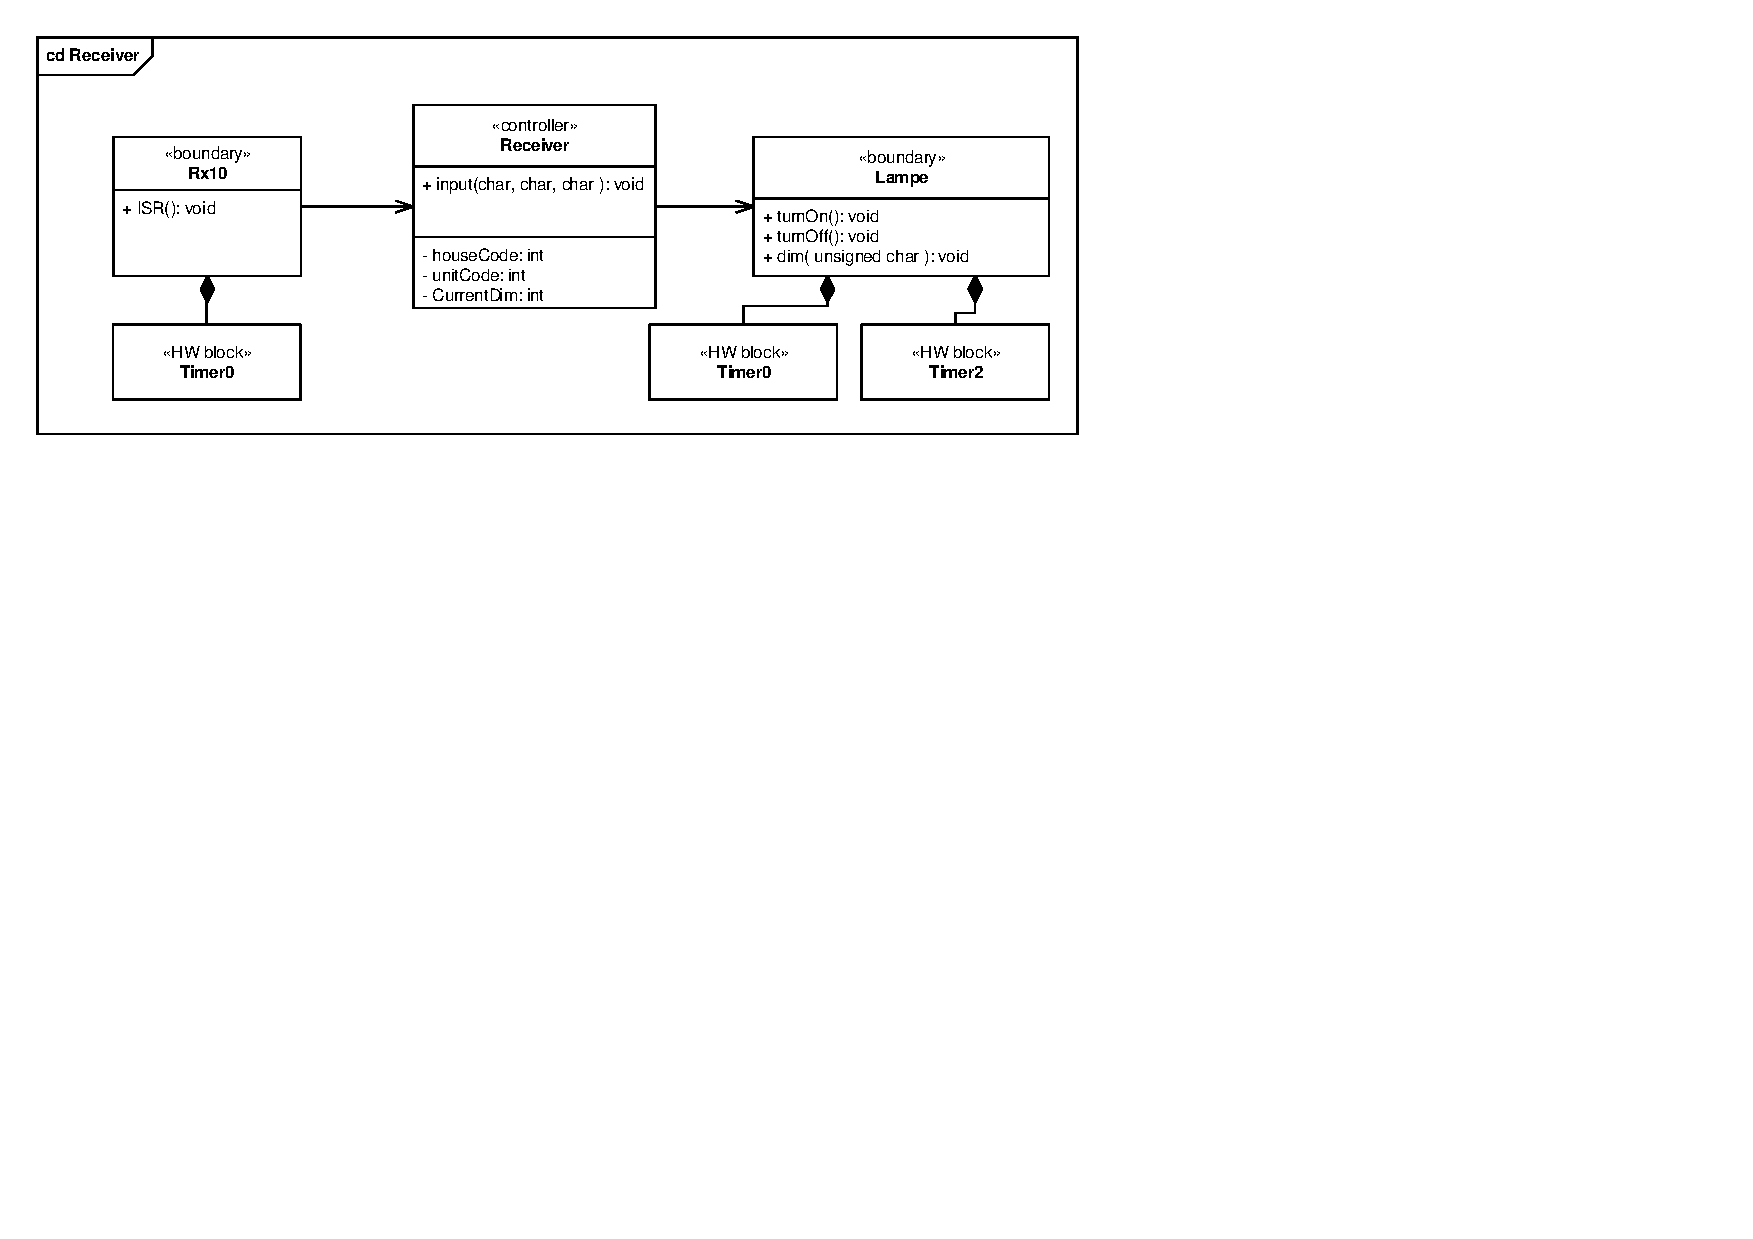
\includegraphics[scale=1,clip=true, trim=38 462 697 66]{Systemarkitektur/diagrammer/Receiver_KlasseDiagram} %L B R T - HUSKE DET
\end{figure}

%ISR
\begin{table}[h]
\begin{tabularx}{\textwidth}{p{0.6 cm} l X} %\hline
\multicolumn{3}{l}{\textbf{ISR}}\\
& Operation: & %Skriv tekst herunder
\texttt{ISR( INT0\_vect )}
\\ & Parametre: & %Skriv tekst herunder
Denne servicerutine er indbygget i Atmega32's IO bibliotek og modtager ingen parametre \cite{lib:AtMega32sum}.
\\ & Beskrivelse: & %Skriv tekst herunder
Denne funktion kaldes ved interrupts på \texttt{PD2 INT0} og skal være \texttt{Friend} af klassen. Ved interrupts skal denne skifte den nuværende værdi på PA0 ind i \texttt{temp}. Der udføres udføres herefter forskellige handlinger afhængigt tilstanden.
\\
\end{tabularx}
\end{table}

%checkData
\begin{table}[h]
\begin{tabularx}{\textwidth}{p{0.6 cm} l X} %\hline
\multicolumn{3}{l}{\textbf{checkData}}\\
& Operation: & %Skriv tekst herunder
\texttt{bool checkData( unsigned char )}
\\ & Parametre: & %Skriv tekst herunder
Modtager 8 nulgennemgange.
\\ & Returværdi: & %Skriv tekst herunder
Returnerer \texttt{TRUE}, hvis de 8 nulgennemgange overholder protokollen for 4 bits og \texttt{FALSE}, hvis den ikke gør.
\\ & Beskrivelse: & %Skriv tekst herunder
Denne metode kontrolleer om en given 4-bit størrelse overholder X.10 protokollen. Der modtages 8 nulgennemgange, som deles op i 4 par. Hvert par udgør 1 bit. For at returnere \texttt{TRUE} skal hvert par bestå af ét 1-tal og ét 0.
\\
\end{tabularx}
\end{table}

%translate
\begin{table}[h]
\begin{tabularx}{\textwidth}{p{0.6 cm} l X} %\hline
\multicolumn{3}{l}{\textbf{translate}}\\
& Operation: & %Skriv tekst herunder
\texttt{unsigned char translate( unsigned char )}
\\ & Parametre: & %Skriv tekst herunder
Modtager en \texttt{char}, som repræsenterer 8 nulgennemgange.
\\ & Returværdi: & %Skriv tekst herunder
Returnerer en \texttt{char} bestående af \texttt{0000} efterfulgt af de 4 bits, som inputtet oversættes til.
\\ & Beskrivelse: & %Skriv tekst herunder
Metoden tager parameteren og oversætter den til 4 bits. For at fylde \texttt{char}'en sættes bit 7-4 til \texttt{0} i returværdien. Bit 3-0 på returværdien sættes til bit 7, 5, 3 og 1 fra parameteren. 
Dvs hvis metoden kaldes med en char \texttt{10011010} vil returværdien være: \texttt{00001011}. 
\\
\end{tabularx}
\end{table}

\begin{table}[h!]
\centering
\begin{tabularx}{13 cm}{|l |X|} \hline
Attribut & Beskrivelse \\ \hline

\texttt{bool start} & Sættes til \texttt{TRUE}, hvis den er igang med at modtage en kommando, ellers sættes den til \texttt{FALSE}. \\ \hline
\texttt{unsigned char count} & Tæller hvor mange nulgennemgange der har været siden sidste hele bit/mønster. \\ \hline
\texttt{unsigned char temp} & Variabel som agerer skifteregister ved modtagelse af nulgennemgange. \\ \hline
\end{tabularx}
\end{table}

\clearpage